% -*- mode: latex; mode: flyspell; ispell-local-dictionary: "en_US"; coding: utf-8; fill-column: 80 -*-

\documentclass{article}

\usepackage[utf8]{inputenc}
\usepackage[english]{babel}

\usepackage{amsmath,amsfonts,amssymb}
\usepackage{fullpage}
\usepackage{verbatim}

\usepackage{tikz,pgfplots}

\pgfplotsset{
  width=150mm,height=100mm,
  major grid style={thin,dotted,color=black!50},
  minor grid style={thin,dotted,color=black!50},
  grid,
  every axis/.append style={
    line width=0.5pt,
    tick style={
      line cap=round,
      thin,
      major tick length=4pt,
      minor tick length=2pt,
    },
  },
  legend cell align=left,
  legend pos=north west,
}

%%%%%%%%%%%%%%%%%%%%%%%%%%%%%%%%%%%%%%%%%%%%%%%%%%%%%%%%%%%%%%%%%%%%%%%%%%%%%%%%

\begin{document}

\title{Speicherplatzanalyse Hashmaps}
\author{}
\maketitle


% IMPORT-DATA mphf stats_mphf_size.txt
% IMPORT-DATA change smaller_tables.txt
% IMPORT-DATA hashmap stats_hashmap_size.txt


\begin{center}
	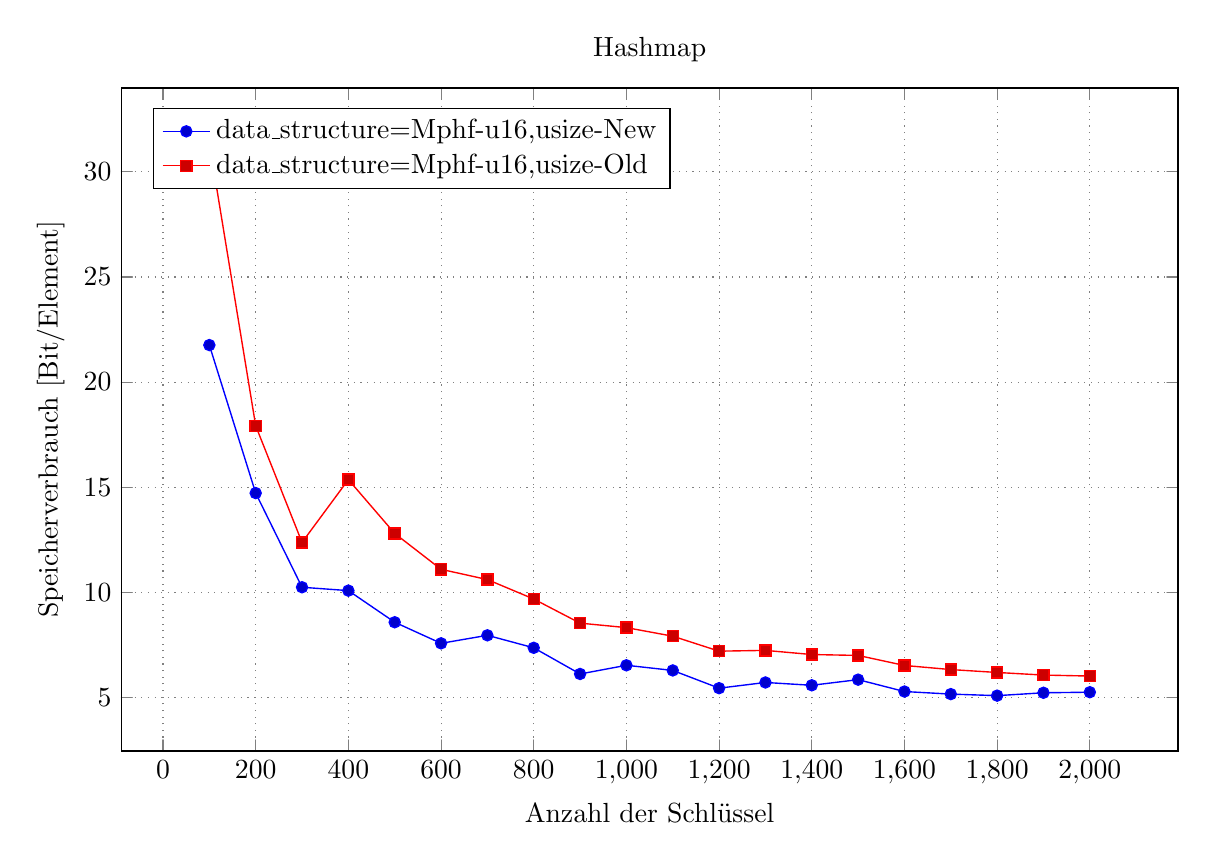
\begin{tikzpicture}
	\begin{axis}[
	title={Hashmap},
	xlabel={Anzahl der Schlüssel},
	ylabel={Speicherverbrauch [Bit/Element]},
	]
	
	%% MULTIPLOT(data_structure) SELECT size AS x, size_bytes AS y, MULTIPLOT
	%% FROM change WHERE x % 100 == 0 and x > 10 GROUP BY MULTIPLOT,x ORDER BY MULTIPLOT,x
 \addplot coordinates { (100,21.76) (200,14.72) (300,10.24) (400,10.08) (500,8.576) (600,7.57333) (700,7.95429) (800,7.36) (900,6.11556) (1000,6.528) (1100,6.28364) (1200,5.44) (1300,5.71077) (1400,5.57714) (1500,5.84533) (1600,5.28) (1700,5.15765) (1800,5.08444) (1900,5.22105) (2000,5.248) };
 \addlegendentry{data\_structure=Mphf-u16,usize-New};
 \addplot coordinates { (100,31.36) (200,17.92) (300,12.3733) (400,15.36) (500,12.8) (600,11.0933) (700,10.6057) (800,9.68) (900,8.53333) (1000,8.32) (1100,7.91273) (1200,7.2) (1300,7.23692) (1400,7.04) (1500,6.99733) (1600,6.52) (1700,6.32471) (1800,6.18667) (1900,6.06316) (2000,6.016) };
 \addlegendentry{data\_structure=Mphf-u16,usize-Old};
	
	
	
	
	
	\end{axis}
	\end{tikzpicture}
\end{center}

\begin{center}
	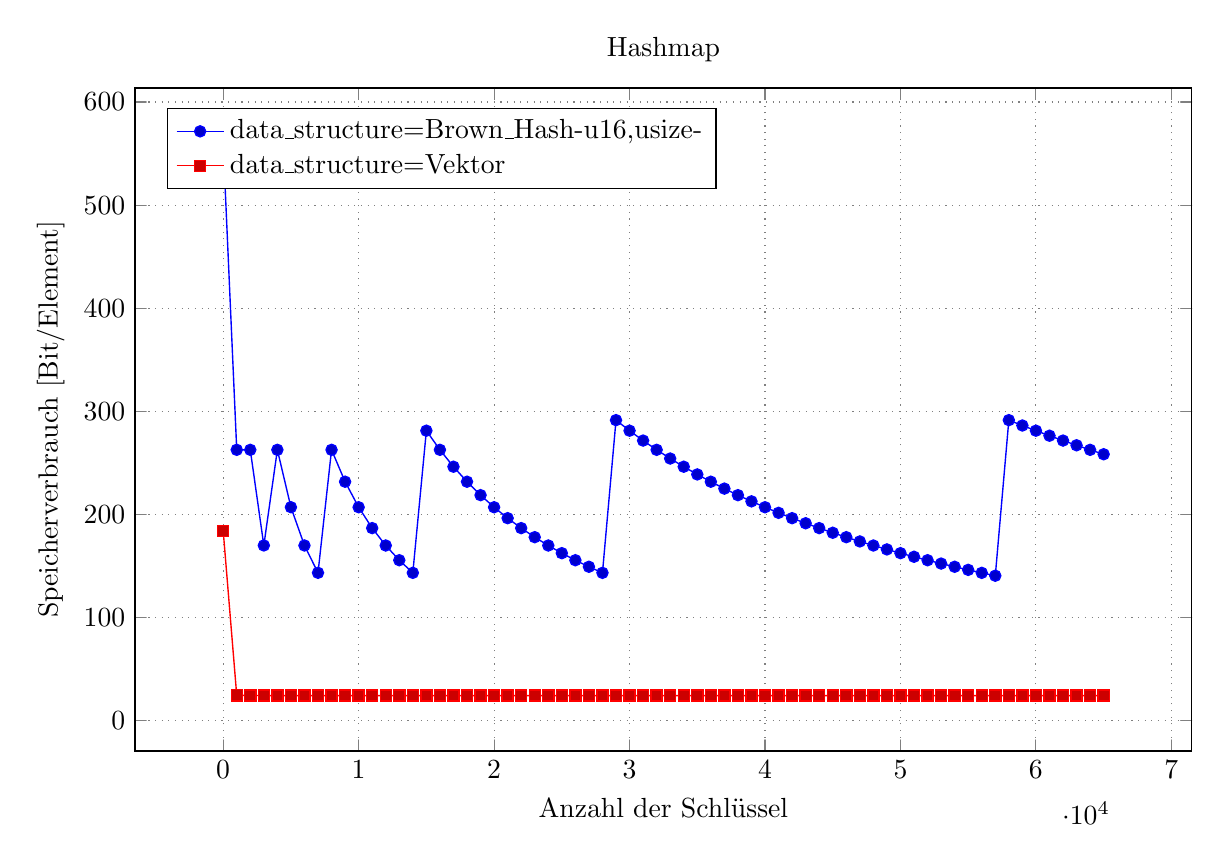
\begin{tikzpicture}
	\begin{axis}[
	title={Hashmap},
	xlabel={Anzahl der Schlüssel},
	ylabel={Speicherverbrauch [Bit/Element]},
	]
	
	%% MULTIPLOT(data_structure) SELECT size AS x, size_bytes AS y, MULTIPLOT
	%% FROM hashmap WHERE x % 1000 == 2  GROUP BY MULTIPLOT,x ORDER BY MULTIPLOT,x
 \addplot coordinates { (2,560.0) (1002,262.547) (2002,262.537) (3002,169.753) (4002,262.533) (5002,206.848) (6002,169.719) (7002,143.196) (8002,262.53) (9002,231.589) (10002,206.835) (11002,186.581) (12002,169.702) (13002,155.42) (14002,143.177) (15002,281.095) (16002,262.529) (17002,246.147) (18002,231.585) (19002,218.556) (20002,206.829) (21002,196.219) (22002,186.574) (23002,177.767) (24002,169.694) (25002,162.267) (26002,155.411) (27002,149.063) (28002,143.168) (29002,291.34) (30002,281.096) (31002,271.513) (32002,262.529) (33002,254.089) (34002,246.146) (35002,238.656) (36002,231.583) (37002,224.892) (38002,218.553) (39002,212.539) (40002,206.826) (41002,201.391) (42002,196.215) (43002,191.28) (44002,186.57) (45002,182.068) (46002,177.763) (47002,173.64) (48002,169.69) (49002,165.9) (50002,162.262) (51002,158.767) (52002,155.406) (53002,152.172) (54002,149.058) (55002,146.057) (56002,143.163) (57002,140.371) (58002,291.341) (59002,286.132) (60002,281.096) (61002,276.226) (62002,271.513) (63002,266.949) (64002,262.528) (65002,258.243) };
 \addlegendentry{data\_structure=Brown\_Hash-u16,usize-};
 \addplot coordinates { (2,184.0) (1002,24.3194) (2002,24.1598) (3002,24.1066) (4002,24.08) (5002,24.064) (6002,24.0533) (7002,24.0457) (8002,24.04) (9002,24.0355) (10002,24.032) (11002,24.0291) (12002,24.0267) (13002,24.0246) (14002,24.0229) (15002,24.0213) (16002,24.02) (17002,24.0188) (18002,24.0178) (19002,24.0168) (20002,24.016) (21002,24.0152) (22002,24.0145) (23002,24.0139) (24002,24.0133) (25002,24.0128) (26002,24.0123) (27002,24.0119) (28002,24.0114) (29002,24.011) (30002,24.0107) (31002,24.0103) (32002,24.01) (33002,24.0097) (34002,24.0094) (35002,24.0091) (36002,24.0089) (37002,24.0086) (38002,24.0084) (39002,24.0082) (40002,24.008) (41002,24.0078) (42002,24.0076) (43002,24.0074) (44002,24.0073) (45002,24.0071) (46002,24.007) (47002,24.0068) (48002,24.0067) (49002,24.0065) (50002,24.0064) (51002,24.0063) (52002,24.0062) (53002,24.006) (54002,24.0059) (55002,24.0058) (56002,24.0057) (57002,24.0056) (58002,24.0055) (59002,24.0054) (60002,24.0053) (61002,24.0052) (62002,24.0052) (63002,24.0051) (64002,24.005) (65002,24.0049) };
 \addlegendentry{data\_structure=Vektor};


	
	
	\end{axis}
	\end{tikzpicture}
\end{center}


\begin{center}
	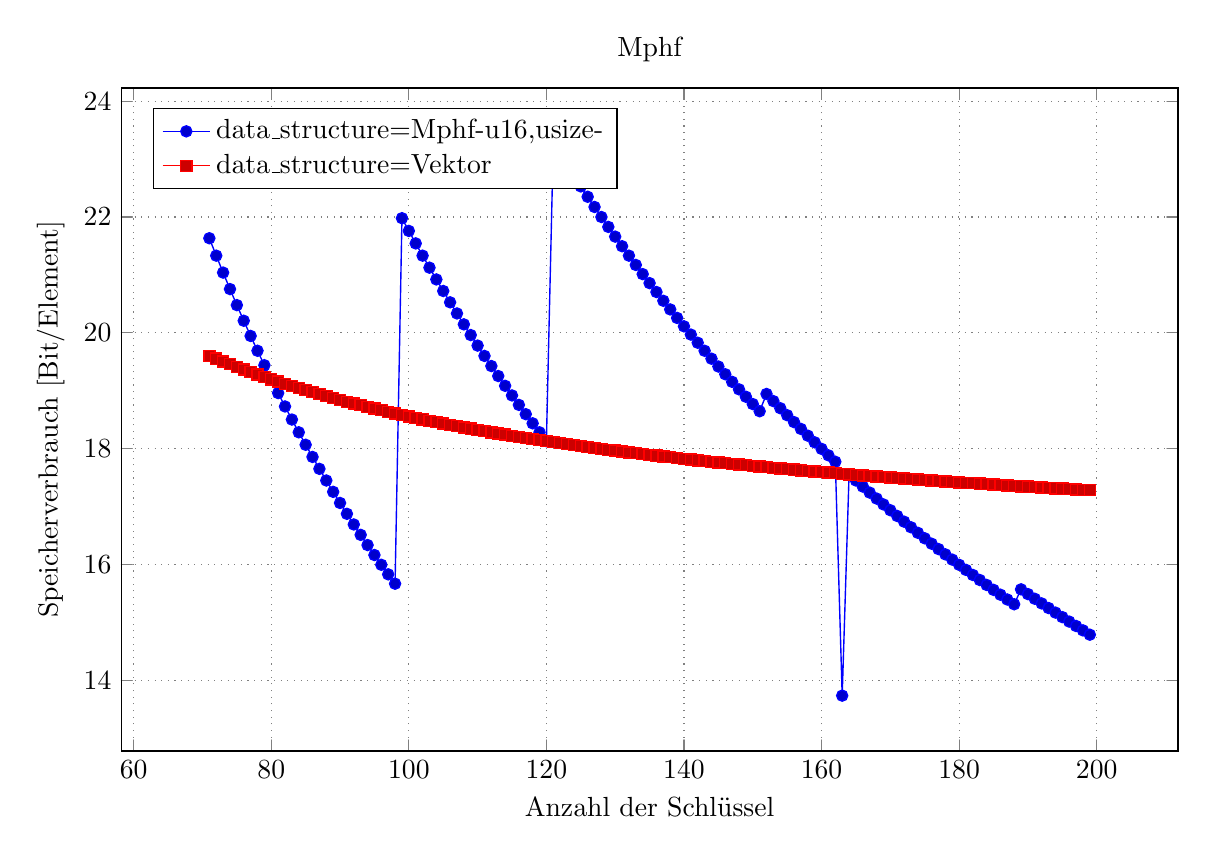
\begin{tikzpicture}
	\begin{axis}[
	title={Mphf},
	xlabel={Anzahl der Schlüssel},
	ylabel={Speicherverbrauch [Bit/Element]},
	]
	
	%% MULTIPLOT(data_structure) SELECT size AS x, size_bytes AS y, MULTIPLOT
	%% FROM mphf WHERE x > 70 AND x < 200 GROUP BY MULTIPLOT,x ORDER BY MULTIPLOT,x
 \addplot coordinates { (71,21.6338) (72,21.3333) (73,21.0411) (74,20.7568) (75,20.48) (76,20.2105) (77,19.9481) (78,19.6923) (79,19.443) (80,19.2) (81,18.963) (82,18.7317) (83,18.506) (84,18.2857) (85,18.0706) (86,17.8605) (87,17.6552) (88,17.4545) (89,17.2584) (90,17.0667) (91,16.8791) (92,16.6957) (93,16.5161) (94,16.3404) (95,16.1684) (96,16.0) (97,15.8351) (98,15.6735) (99,21.9798) (100,21.76) (101,21.5446) (102,21.3333) (103,21.1262) (104,20.9231) (105,20.7238) (106,20.5283) (107,20.3364) (108,20.1481) (109,19.9633) (110,19.7818) (111,19.6036) (112,19.4286) (113,19.2566) (114,19.0877) (115,18.9217) (116,18.7586) (117,18.5983) (118,18.4407) (119,18.2857) (120,18.1333) (121,23.2727) (122,23.082) (123,22.8943) (124,22.7097) (125,22.528) (126,22.3492) (127,22.1732) (128,22.0) (129,21.8295) (130,21.6615) (131,21.4962) (132,21.3333) (133,21.1729) (134,21.0149) (135,20.8593) (136,20.7059) (137,20.5547) (138,20.4058) (139,20.259) (140,20.1143) (141,19.9716) (142,19.831) (143,19.6923) (144,19.5556) (145,19.4207) (146,19.2877) (147,19.1565) (148,19.027) (149,18.8993) (150,18.7733) (151,18.649) (152,18.9474) (153,18.8235) (154,18.7013) (155,18.5806) (156,18.4615) (157,18.3439) (158,18.2278) (159,18.1132) (160,18.0) (161,17.8882) (162,17.7778) (163,13.7423) (164,17.561) (165,17.4545) (166,17.3494) (167,17.2455) (168,17.1429) (169,17.0414) (170,16.9412) (171,16.8421) (172,16.7442) (173,16.6474) (174,16.5517) (175,16.4571) (176,16.3636) (177,16.2712) (178,16.1798) (179,16.0894) (180,16.0) (181,15.9116) (182,15.8242) (183,15.7377) (184,15.6522) (185,15.5676) (186,15.4839) (187,15.4011) (188,15.3191) (189,15.5767) (190,15.4947) (191,15.4136) (192,15.3333) (193,15.2539) (194,15.1753) (195,15.0974) (196,15.0204) (197,14.9442) (198,14.8687) (199,14.794) };
 \addlegendentry{data\_structure=Mphf-u16,usize-};
 \addplot coordinates { (71,19.6056) (72,19.5556) (73,19.5068) (74,19.4595) (75,19.4133) (76,19.3684) (77,19.3247) (78,19.2821) (79,19.2405) (80,19.2) (81,19.1605) (82,19.122) (83,19.0843) (84,19.0476) (85,19.0118) (86,18.9767) (87,18.9425) (88,18.9091) (89,18.8764) (90,18.8444) (91,18.8132) (92,18.7826) (93,18.7527) (94,18.7234) (95,18.6947) (96,18.6667) (97,18.6392) (98,18.6122) (99,18.5859) (100,18.56) (101,18.5347) (102,18.5098) (103,18.4854) (104,18.4615) (105,18.4381) (106,18.4151) (107,18.3925) (108,18.3704) (109,18.3486) (110,18.3273) (111,18.3063) (112,18.2857) (113,18.2655) (114,18.2456) (115,18.2261) (116,18.2069) (117,18.188) (118,18.1695) (119,18.1513) (120,18.1333) (121,18.1157) (122,18.0984) (123,18.0813) (124,18.0645) (125,18.048) (126,18.0317) (127,18.0157) (128,18.0) (129,17.9845) (130,17.9692) (131,17.9542) (132,17.9394) (133,17.9248) (134,17.9104) (135,17.8963) (136,17.8824) (137,17.8686) (138,17.8551) (139,17.8417) (140,17.8286) (141,17.8156) (142,17.8028) (143,17.7902) (144,17.7778) (145,17.7655) (146,17.7534) (147,17.7415) (148,17.7297) (149,17.7181) (150,17.7067) (151,17.6954) (152,17.6842) (153,17.6732) (154,17.6623) (155,17.6516) (156,17.641) (157,17.6306) (158,17.6203) (159,17.6101) (160,17.6) (161,17.5901) (162,17.5802) (163,17.5706) (164,17.561) (165,17.5515) (166,17.5422) (167,17.5329) (168,17.5238) (169,17.5148) (170,17.5059) (171,17.4971) (172,17.4884) (173,17.4798) (174,17.4713) (175,17.4629) (176,17.4545) (177,17.4463) (178,17.4382) (179,17.4302) (180,17.4222) (181,17.4144) (182,17.4066) (183,17.3989) (184,17.3913) (185,17.3838) (186,17.3763) (187,17.369) (188,17.3617) (189,17.3545) (190,17.3474) (191,17.3403) (192,17.3333) (193,17.3264) (194,17.3196) (195,17.3128) (196,17.3061) (197,17.2995) (198,17.2929) (199,17.2864) };
 \addlegendentry{data\_structure=Vektor};
 
 
	
	\end{axis}
	\end{tikzpicture}
\end{center}




\end{document}

%%%%%%%%%%%%%%%%%%%%%%%%%%%%%%%%%%%%%%%%%%%%%%%%%%%%%%%%%%%%%%%%%%%%%%%%%%%%%%%%
